\textbf{Пример 1}

Для дороги, показанной на рисунке ниже, будет сделан следующей вызов функции:

\texttt{find\_shortcut(4, [10, 20, 20], [0, 40, 0, 30], 10)}

Оптимальное решение~--- построить экспресс-линию между станциями $1$ и $3$, как показано ниже.

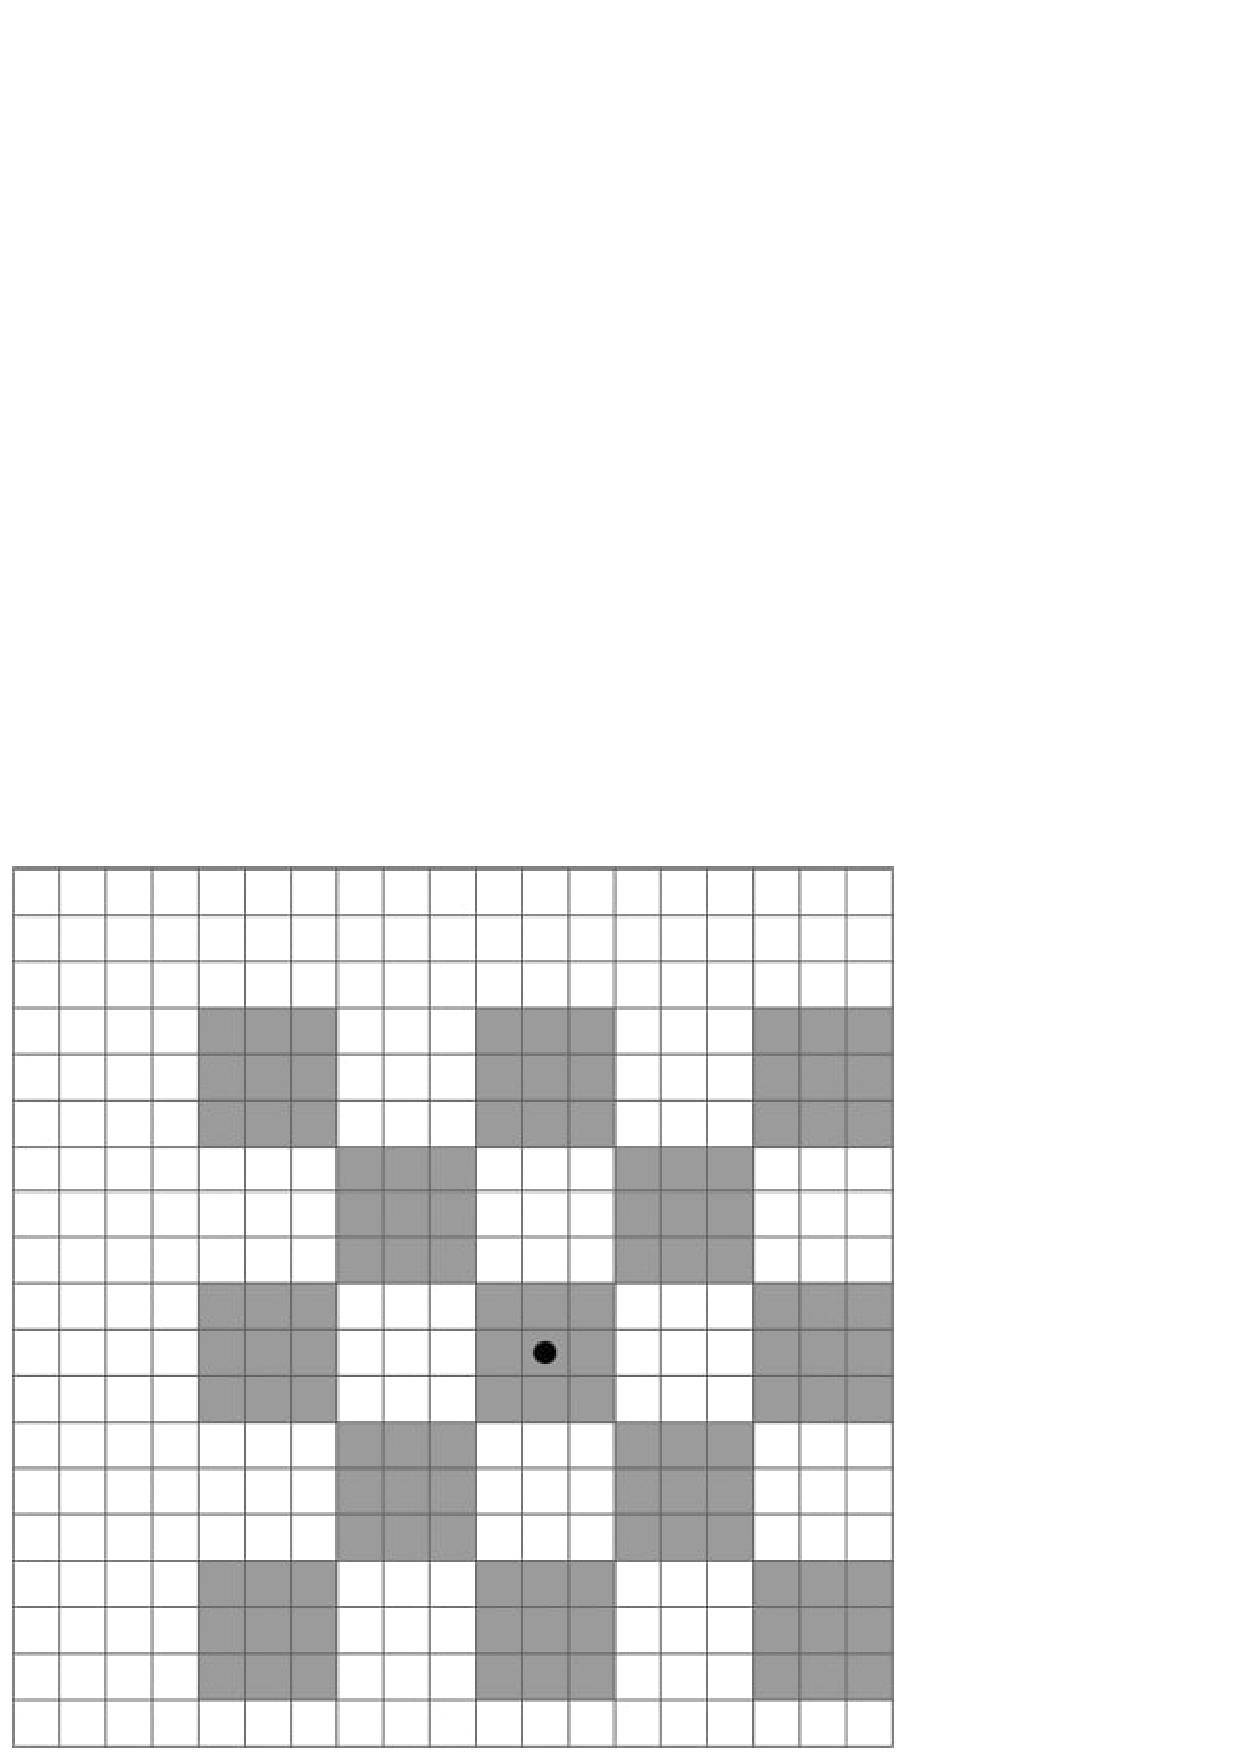
\includegraphics[scale=0.9]{2.png}

Диаметр получившейся железнодорожной дороги равен $80$ сантиметрам, поэтому функция должна вернуть $80$.

\textbf{Пример 2}

Если будет сделан вызов функции:

\texttt{find\_shortcut(9, [10, 10, 10, 10, 10, 10, 10, 10], [20, 0, 30, 0, 0, 40, 0, 40, 0], 30)}

Оптимальное решение~--- соединить станции $2$ и $7$, в этом случае диаметр
равен $110$.

\textbf{Пример 3}

Если будет сделан вызов функции:

\texttt{find\_shortcut(4, [2, 2, 2], [1, 10, 10, 1], 1) }

Оптимальное решение~--- соединить станции $1$ и $2$, уменьшая диаметр до $21$.

\textbf{Пример 4}

Если будет сделан вызов функции:

\texttt{find\_shortcut(3, [1, 1], [1, 1, 1], 3)}

Соединение любых двух станций экспресс-линией длины $3$ не уменьшает
изначальный диаметр железнодорожной сети равный $4$.
